%!TEX TS-program = xelatex

% Шаблон документа LaTeX создан в 2018 году
% Алексеем Подчезерцевым
% В качестве исходных использованы шаблоны
% 	Данилом Фёдоровых (danil@fedorovykh.ru) 
%		https://www.writelatex.com/coursera/latex/5.2.2
%	LaTeX-шаблон для русской кандидатской диссертации и её автореферата.
%		https://github.com/AndreyAkinshin/Russian-Phd-LaTeX-Dissertation-Template

\documentclass[a4paper,14pt]{article}

%%% Работа с русским языком
\usepackage[english,russian]{babel}   %% загружает пакет многоязыковой вёрстки
\usepackage{fontspec}      %% подготавливает загрузку шрифтов Open Type, True Type и др.
\defaultfontfeatures{Ligatures={TeX},Renderer=Basic}  %% свойства шрифтов по умолчанию
\setmainfont[Ligatures={TeX,Historic}]{Times New Roman} %% задаёт основной шрифт документа
\setsansfont{Comic Sans MS}                    %% задаёт шрифт без засечек
\setmonofont{Courier New}
\usepackage{indentfirst}
\frenchspacing

\renewcommand{\epsilon}{\ensuremath{\varepsilon}}
\renewcommand{\phi}{\ensuremath{\varphi}}
\renewcommand{\kappa}{\ensuremath{\varkappa}}
\renewcommand{\le}{\ensuremath{\leqslant}}
\renewcommand{\leq}{\ensuremath{\leqslant}}
\renewcommand{\ge}{\ensuremath{\geqslant}}
\renewcommand{\geq}{\ensuremath{\geqslant}}
\renewcommand{\emptyset}{\varnothing}

%%% Дополнительная работа с математикой
\usepackage{amsmath,amsfonts,amssymb,amsthm,mathtools} % AMS
\usepackage{icomma} % "Умная" запятая: $0,2$ --- число, $0, 2$ --- перечисление

%% Номера формул
%\mathtoolsset{showonlyrefs=true} % Показывать номера только у тех формул, на которые есть \eqref{} в тексте.
%\usepackage{leqno} % Нумерация формул слева	

%% Перенос знаков в формулах (по Львовскому)
\newcommand*{\hm}[1]{#1\nobreak\discretionary{}
{\hbox{$\mathsurround=0pt #1$}}{}}

%%% Работа с картинками
\usepackage{graphicx}  % Для вставки рисунков
\graphicspath{{images/}}  % папки с картинками
\setlength\fboxsep{3pt} % Отступ рамки \fbox{} от рисунка
\setlength\fboxrule{1pt} % Толщина линий рамки \fbox{}
\usepackage{wrapfig} % Обтекание рисунков текстом

%%% Работа с таблицами
\usepackage{array,tabularx,tabulary,booktabs} % Дополнительная работа с таблицами
\usepackage{longtable}  % Длинные таблицы
\usepackage{multirow} % Слияние строк в таблице
\usepackage{float}% http://ctan.org/pkg/float

%%% Программирование
\usepackage{etoolbox} % логические операторы


%%% Страница
\usepackage{extsizes} % Возможность сделать 14-й шрифт
\usepackage{geometry} % Простой способ задавать поля
\geometry{top=20mm}
\geometry{bottom=20mm}
\geometry{left=20mm}
\geometry{right=10mm}
%
%\usepackage{fancyhdr} % Колонтитулы
% 	\pagestyle{fancy}
%\renewcommand{\headrulewidth}{0pt}  % Толщина линейки, отчеркивающей верхний колонтитул
% 	\lfoot{Нижний левый}
% 	\rfoot{Нижний правый}
% 	\rhead{Верхний правый}
% 	\chead{Верхний в центре}
% 	\lhead{Верхний левый}
%	\cfoot{Нижний в центре} % По умолчанию здесь номер страницы

\usepackage{setspace} % Интерлиньяж
\onehalfspacing % Интерлиньяж 1.5
%\doublespacing % Интерлиньяж 2
%\singlespacing % Интерлиньяж 1

\usepackage{lastpage} % Узнать, сколько всего страниц в документе.

\usepackage{soul} % Модификаторы начертания

\usepackage{hyperref}
\usepackage[usenames,dvipsnames,svgnames,table,rgb]{xcolor}
\hypersetup{                % Гиперссылки
unicode=true,           % русские буквы в раздела PDF
pdftitle={Заголовок},   % Заголовок
pdfauthor={Автор},      % Автор
pdfsubject={Тема},      % Тема
pdfcreator={Создатель}, % Создатель
pdfproducer={Производитель}, % Производитель
pdfkeywords={keyword1}, % Ключевые слова
colorlinks=true,        % false: ссылки в рамках; true: цветные ссылки
linkcolor=black,          % внутренние ссылки
citecolor=black,        % на библиографию
filecolor=magenta,      % на файлы
urlcolor=blue           % на URL
}
\makeatletter
\def\@biblabel#1{#1. }
\makeatother
\usepackage{cite} % Работа с библиографией
%\usepackage[superscript]{cite} % Ссылки в верхних индексах
%\usepackage[nocompress]{cite} % 
\usepackage{csquotes} % Еще инструменты для ссылок

\usepackage{multicol} % Несколько колонок

\usepackage{tikz} % Работа с графикой
\usepackage{pgfplots}
\usepackage{pgfplotstable}

% ГОСТ заголовки
\usepackage[font=small]{caption}
%\captionsetup[table]{justification=centering, labelsep = newline} % Таблицы по правобу краю
%\captionsetup[figure]{justification=centering} % Картинки по центру


\newcommand{\tablecaption}[1]{\addtocounter{table}{1}\small \begin{flushright}
                                                                \tablename \ \thetable
\end{flushright}%
\begin{center}
    #1
\end{center}}

\newcommand{\imref}[1]{рис.~\ref{#1}}

\usepackage{multirow}
\usepackage{spreadtab}
\newcolumntype{K}[1]{@{}>{\centering\arraybackslash}p{#1cm}@{}}


\usepackage{xparse}
\usepackage{fancyvrb}

\RecustomVerbatimCommand{\VerbatimInput}{VerbatimInput}
{
fontsize=\footnotesize
}

\usepackage{tocloft}
\renewcommand{\cftsecleader}{\cftdotfill{\cftdotsep}}
\begin{document} % конец преамбулы, начало документа
    \begin{titlepage}
    \begin{center}
        ФЕДЕРАЛЬНОЕ ГОСУДАРСТВЕННОЕ АВТОНОМНОЕ \\
        ОБРАЗОВАТЕЛЬНОЕ УЧРЕЖДЕНИЕ ВЫСШЕГО ОБРАЗОВАНИЯ\\
        «НАЦИОНАЛЬНЫЙ ИССЛЕДОВАТЕЛЬСКИЙ УНИВЕРСИТЕТ\\
        «ВЫСШАЯ ШКОЛА ЭКОНОМИКИ»
    \end{center}

    \begin{center}
        \textbf{Московский институт электроники и математики}

        \textbf{им. А.Н.Тихонова НИУ ВШЭ}

        \vspace{2ex}

        \textbf{Департамент компьютерной инженерии}
    \end{center}
    \vspace{1ex}

    \begin{center}
        Курс «Высокоуровневое и имитационное моделирование цифровых систем»
    \end{center}


    \begin{center}
        \textbf{ОТЧЕТ\\
        ПО ЛАБОРАТОРНОЙ РАБОТЕ №3
        }
    \end{center}

    \begin{center}
        Тема работы: «Реализация нейронной сети MobileNet на ПЛИС»
    \end{center}

    \vspace{2ex}

    \begin{flushright}
        \textbf{Выполнили:}

        \vspace{2ex}

        Студенты группы БИВ174

        Бригада №5

        \vspace{2ex}

        Подчезерцев Алексей Евгеньевич

        Солодянкин Андрей Александрович
        \vspace{2ex}

        \textbf{Принял:}

        асс. МИЭМ НИУ ВШЭ

        Американов А.А.

    \end{flushright}

    \vfill
    \begin{center}
        Москва \the\year \, г.
    \end{center}

\end{titlepage}
\addtocounter{page}{1}
    \tableofcontents
    \pagebreak


    \section{Задание}

    Бригада №5, вариант 1, плата DE10-nano.

    \begin{enumerate}
        \item Разработать на высокоуровневом языке программирования модель сети Хебба, способную распознать не менее 8 различных букв;
        \item Разработать модель нейрона на Verilog, произвести моделирование;
        \item Объединить нейроны, определить точность распознавания;
        \item Определить зависимость потребления ресурсов от количества нейронов;
        \item Выполнить прототипирование сети.
    \end{enumerate}


    \section{Выполнение работы}

    \subsection{Разработка сети}

    Была создана модель сети Хебба с помощью языка программирования Python.
    Низким уровнем сигнала был принят 0, а высоким -- 1.
    Кроме того, была написана дополнительная логика для сохранения полученной модели в код на Verilog,
    а так же проверки на переполнение полученной модели.

    Исходный код нейрона:
    {\small \VerbatimInput{../hebbian_net_lab_02/net/neuron.py}}

    Исходный код слоя:
    {\small \VerbatimInput{../hebbian_net_lab_02/net/layers.py}}

    Исходный код модели:
    {\small \VerbatimInput{../hebbian_net_lab_02/net/models.py}}

    Исходный код верхнеуровневого модуля:
    {\small \VerbatimInput{../hebbian_net_lab_02/example_03.py}}

    Результат запуска:
    {\small \VerbatimInput{logs/example_03.txt}}

    Программа отображает прогресс выполнения и может индицировать о досрочном завершении.
    После отображается ожидаемое и предсказанное значение для каждого символа и сам символ.
    В самом конце генерируется фрагмент кода для тестирования устройства.
    Созданный код нейрона и веса автоматически сохраняются после обучения.

    \subsection{Разработка сети на Verilog}

    Полученный код нейрона на языке Verilog:
    {\small \VerbatimInput{../de10-nano/neuron.v}}
    Для подсчета суммы использовалась оптимизация, которая позволяет сократить длительность подсчета суммы с линейного времени от размера изображения до логарифма от этого значения.
    Кроме того, операция умножения была заменена тернарным оператором, так как всего возможно 2 ситуации -- умножение на 0 и на 1.
    В первом случае результат 0, в другом -- то же самое число.
    Результат симуляции малой версии нейрона на примере из методических указаний представлен на рис.~\ref{fig:sim_small}.

    \begin{figure}[H]
        \centering
        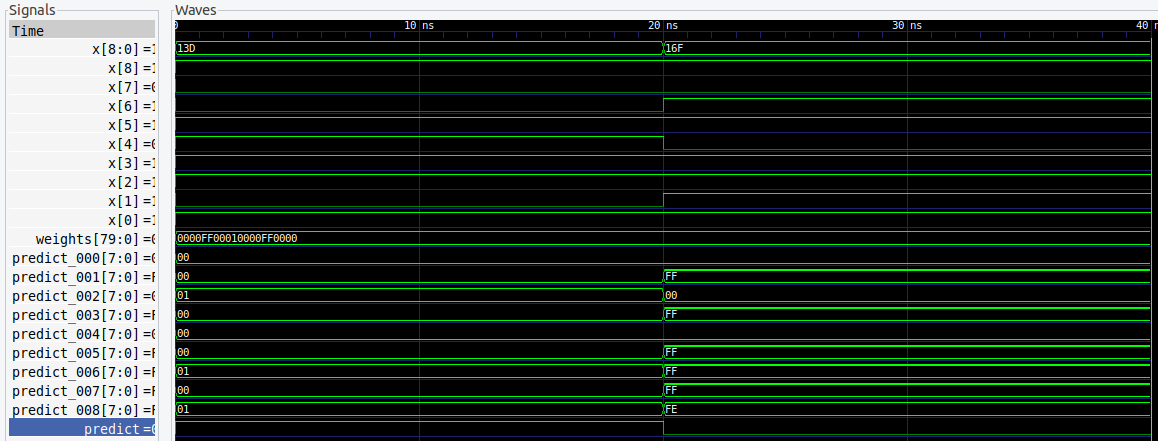
\includegraphics[width=\linewidth]{images/sim_small}
        \caption{Симуляция малого нейрона}
        \label{fig:sim_small}
    \end{figure}

    \subsection{Объединение нейронов}

    Было выполнено объединение нейронов с помощью конструкции generate.
    Однако, симулятор Icarus Verilog требовал имени для каждого инстанса нейрона, поэтому цикл был развернут вручную.

    {\small \VerbatimInput{../de10-nano/layer.v}}

    Было проведена симуляция и тестирование сети (рис.~\ref{fig:sim_test}).
    По результатам тестирования предсказание сети на Python совпало с результатом симуляции Verilog,
    то есть сеть идеально распознавала элементы.
    Такое высокое качество было достигнуто за счёт подбора хорошей разметки.
    Стандартные варианты разметки не давали приличного качества даже на высокоуровневых языках.
    Это связано с несовершенствами сети Хебба.

    \begin{figure}[H]
        \centering
        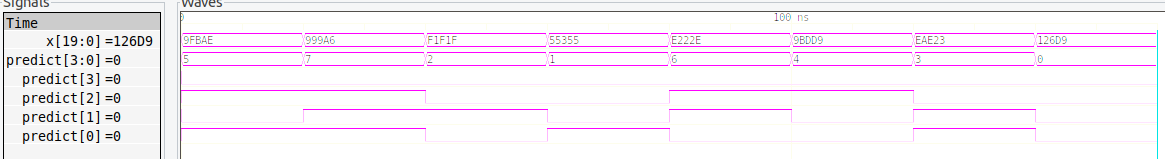
\includegraphics[width=\linewidth]{images/sim_test}
        \caption{Симуляция слоя сети}
        \label{fig:sim_test}
    \end{figure}

    \subsection{Потребление ресурсов}
    Итоговая схема потребляет 1 логический элемент.
    На каждый пиксель изображения и на каждый выход сети расходуется по 1 пину.
    На сеть с 100 выходов тратится 120 пинов и 1 логический элемент (рис.~\ref{fig:plot}).
    \begin{figure}[H]
        \centering
        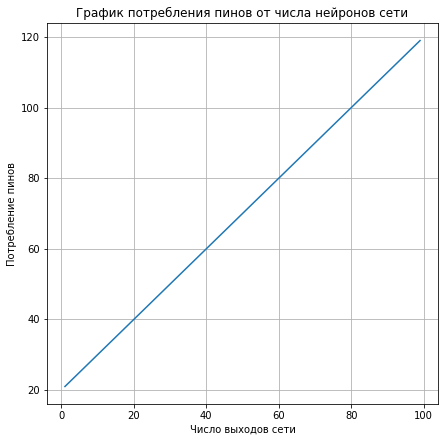
\includegraphics[width=0.5\linewidth]{images/plot}
        \caption{Потребление ресурсов}
        \label{fig:plot}
    \end{figure}


    \section{Исходные коды}

    Исходные коды доступны на \href{https://github.com/AsciiShell/hse_hlimds_labs}
    {https://github.com/AsciiShell/hse\_hlimds\_labs}.

    Pull request работы \href{https://github.com/AsciiShell/hse_hlimds_labs/pull/2}
    {https://github.com/AsciiShell/hse\_hlimds\_labs/pull/2}.

    Релизы \href{https://github.com/AsciiShell/hse_hlimds_labs/releases}
    {https://github.com/AsciiShell/hse\_hlimds\_labs/releases}.


    \section{Выводы по работе}
    В ходе работы была изучена сеть Хебба, разобран принцип ее работы, особенности обучения сети.
    Были подобраны изображения и разметка, позволяющая идеально точно выполнять работу сети.
    Была создана программа, позволяющая перенести обученную сеть на Verilog.
    Проведено тестирование сети, получены результаты точности распознавания, потребления ресурсов.
    Итоговый вариант был записан на плату.

\end{document} % конец документа
